\documentclass[noinstructornotes]{ximera}
%handout:  for handout version with no solutions or instructor notes
%handout,instructornotes:  for instructor version with just problems and notes, no solutions
%noinstructornotes:  shows only problem and solutions

%% handout
%% space
%% newpage
%% numbers
%% nooutcomes

%I added the commands here so that I would't have to keep looking them up
%\newcommand{\RR}{\mathbb R}
%\renewcommand{\d}{\,d}
%\newcommand{\dd}[2][]{\frac{d #1}{d #2}}
%\renewcommand{\l}{\ell}
%\newcommand{\ddx}{\frac{d}{dx}}
%\everymath{\displaystyle}
%\newcommand{\dfn}{\textbf}
%\newcommand{\eval}[1]{\bigg[ #1 \bigg]}

%\begin{image}
%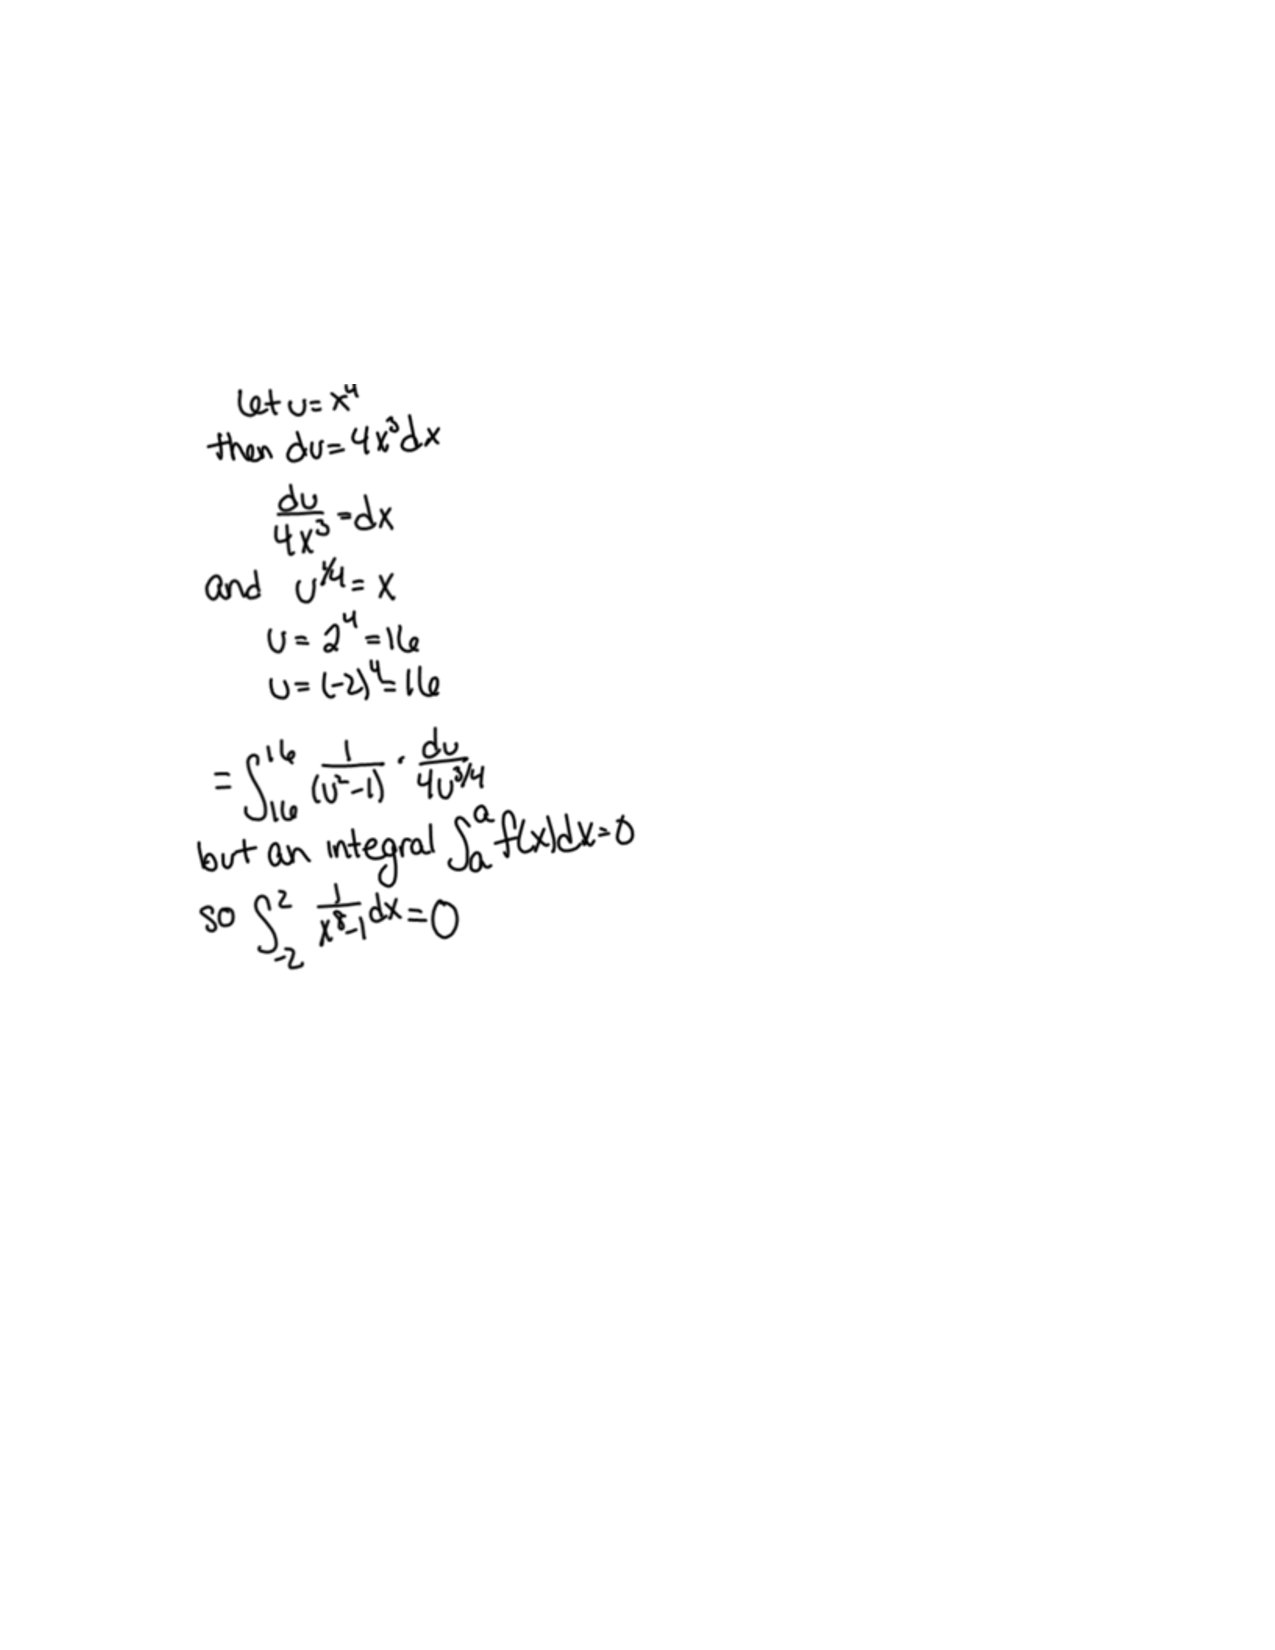
\includegraphics[trim= 170 420 250 180]{Figure1.pdf}
%\end{image}

%add a ``.'' below when used in a specific directory.
\newcommand{\RR}{\mathbb R}
\renewcommand{\d}{\,d}
\newcommand{\dd}[2][]{\frac{d #1}{d #2}}
\renewcommand{\l}{\ell}
\newcommand{\ddx}{\frac{d}{dx}}
\newcommand{\dfn}{\textbf}
\newcommand{\eval}[1]{\bigg[ #1 \bigg]}

\usepackage{multicol}

\renewenvironment{freeResponse}{
\ifhandout\setbox0\vbox\bgroup\else
\begin{trivlist}\item[\hskip \labelsep\bfseries Solution:\hspace{2ex}]
\fi}
{\ifhandout\egroup\else
\end{trivlist}
\fi} %% we can turn off input when making a master document

\title{Recitation \#10: Trigonometric substitutions - Solutions}  

\begin{document}
\begin{abstract}		\end{abstract}
\maketitle



\begin{comment}
\section{Warm up:}

	\begin{freeResponse}
	
	\end{freeResponse}
	
\begin{instructorNotes}

\end{instructorNotes}
\end{comment}







\section{Group work:}



%problem 1
\begin{problem}
Evaluate the following integrals
	\begin{enumerate}
	\item 
	\[
	\int \limits_{ -\frac{5}{3}}^{-\frac{5}{6}} \frac{\sqrt{36x^2-25}}{x^3} \d x.
	\]
	\begin{freeResponse}
	First notice that
		\begin{align*}
		\sqrt{36x^2-25} &= 5\sqrt{\frac{36x^2}{25} - 1}  \\
		&= 5\sqrt{\left( \frac{6x}{5} \right)^2 - 1}.
		\end{align*}
	So we substitute
		\[
		\frac{6x}{5} = \sec \theta	\qquad	\Longrightarrow	\qquad	x = \frac{5}{6} \sec \theta
		\]
	which gives
		\[
		\d x = \frac{5}{6} \sec \theta \tan \theta \d \theta  .
		\]
	Also, notice that
		\begin{itemize}
		\item when $x = - \frac{5}{3}$:
			\[
			-\frac{5}{3} = \frac{5}{6} \sec \theta \qquad	\Longrightarrow \qquad 	\sec \theta = 2 	\qquad 	\Longrightarrow 	\qquad	\theta = \frac{2\pi}{3}
			\]
			
		\item and when $x=-\frac{5}{6}$:\
			\[
			-\frac{5}{6} = \frac{5}{6} \sec \theta	\qquad	\Longrightarrow	\qquad	\sec \theta = -1	\qquad	\Longrightarrow	\qquad	\theta = \pi.
			\]
		\end{itemize}

	Therefore
		\begin{align*}
		\int_{-\frac{5}{3}}^{-\frac{5}{6}} \frac{\sqrt{36x^2-25}}{x^3} \d x 
		&= 5 \int_{\frac{2\pi}{3}}^{\pi} \frac{\sqrt{\sec^2 \theta - 1}}{\left( \frac{5}{6} \sec \theta \right)^3} \left( \frac{5}{6} \sec \theta \tan \theta \right) \d \theta  \\
		&= 5 \cdot \left(\frac{6}{5} \right)^2 \int_{\frac{2\pi}{3}}^{\pi} \frac{|\tan \theta| \tan \theta}{\sec^2 \theta} \d \theta .
		\end{align*}
	Now, notice that $\tan \theta < 0$ whenever $\frac{2\pi}{3} \leq \theta \leq \pi$.  
	So $|\tan \theta| = - \tan \theta$.
	We continue:
		\begin{align*}
		5 \cdot \left(\frac{6}{5} \right)^2 \int_{\frac{2\pi}{3}}^{\pi} \frac{|\tan \theta| \tan \theta}{\sec^2 \theta} \d \theta
		&= - \frac{36}{5} \int_{\frac{2\pi}{3}}^{\pi} \frac{\tan^2 \theta}{\sec^2 \theta} \d \theta  \\
		&= - \frac{36}{5} \int_{\frac{2\pi}{3}}^{\pi} \frac{\sin^2 \theta}{\cos^2 \theta} \cdot \frac{\cos^2 \theta}{1} \d \theta  \\
		&= - \frac{36}{5} \int_{\frac{2\pi}{3}}^{\pi} \sin^2 \theta \d \theta  \\
		&= - \frac{36}{5} \int_{\frac{2\pi}{3}}^{\pi} \frac{1}{2} \left( 1 - \cos (2\theta) \right) \d \theta  \\
		&= - \frac{18}{5} \eval{\theta - \frac{1}{2} \sin (2\theta)}_{\frac{2\pi}{3}}^{\pi}  \\
		&= - \frac{18}{5} \left[ \left( \pi - 0 \right) - \left( \frac{2\pi}{3} + \frac{\sqrt{3}}{4} \right) \right]  
		\qquad {\color{red} \sin \left( \frac{4\pi}{3} \right) = -\frac{\sqrt{3}}{2} }\\
		&= - \frac{18}{5} \left( \frac{\pi}{3} - \frac{\sqrt{3}}{4} \right).
		\end{align*}
	\end{freeResponse}
	
	\item 
	\[
	\int \frac{\d x}{\left( x^2 - 6x + 11 \right)^2}.
	\]
	\begin{freeResponse}
	We begin by completing the square in the denominator
		\[
		x^2 - 6x - 11 = x^2 - 6x + 9 + 2 = (x-3)^2 + 2.
		\]
	We then have that
		\begin{align*}
		\int \frac{\d x}{\left( x^2 - 6x + 11 \right)^2} 
		&= \int \frac{1}{((x-3)^2 + 2)^2} \d x  \\
		&= \frac{1}{4} \int \frac{1}{\left( \frac{(x-3)^2}{2} + 1 \right)^2} \d x  \\
		&= \frac{1}{4} \int \frac{1}{\left( \left( \frac{x-3}{\sqrt{2}} \right)^2 + 1 \right)^2} \d x.
		\end{align*}
	So we substitute
		\begin{equation}\label{substitution1}
		\frac{x-3}{\sqrt{2}} = \tan \theta	\qquad	\Longrightarrow	\qquad	x = \sqrt{2} \tan \theta + 3
		\end{equation}
	and then
		\[
		\d x = \sqrt{2} \sec^2 \theta \d \theta.
		\]
	Continuing with the integral
		\begin{align*}
		\frac{1}{4} \int \frac{1}{\left( \left( \frac{x-3}{\sqrt{2}} \right)^2 + 1 \right)^2} \d x
		&= \frac{1}{4} \int \frac{1}{\left( \tan^2 \theta + 1 \right)^2} \sqrt{2} \sec^2 \theta \d \theta  \\
		&= \frac{\sqrt{2}}{4} \int \frac{1}{\sec^2 \theta} \d \theta  \\
		&= \frac{\sqrt{2}}{4} \int \cos^2 \theta \d \theta  \\
		&= \frac{\sqrt{2}}{4} \int \frac{1}{2} \left( 1 + \cos(2\theta) \right) \d \theta  \\
		&= \frac{\sqrt{2}}{8} \left( \theta + \frac{1}{2} \sin(2\theta) \right) + C .
		\end{align*}
	Now all that is left to do is to reverse-substitute for $\theta$.  
	First, from equation \eqref{substitution1} we have that
		\[
		\theta = \arctan \left( \frac{x-3}{\sqrt{2}} \right).
		\]
	Now, we again use equation \eqref{substitution1} along with Pythagorean's Theorem to construct the following triangle.
	
		\begin{image}
		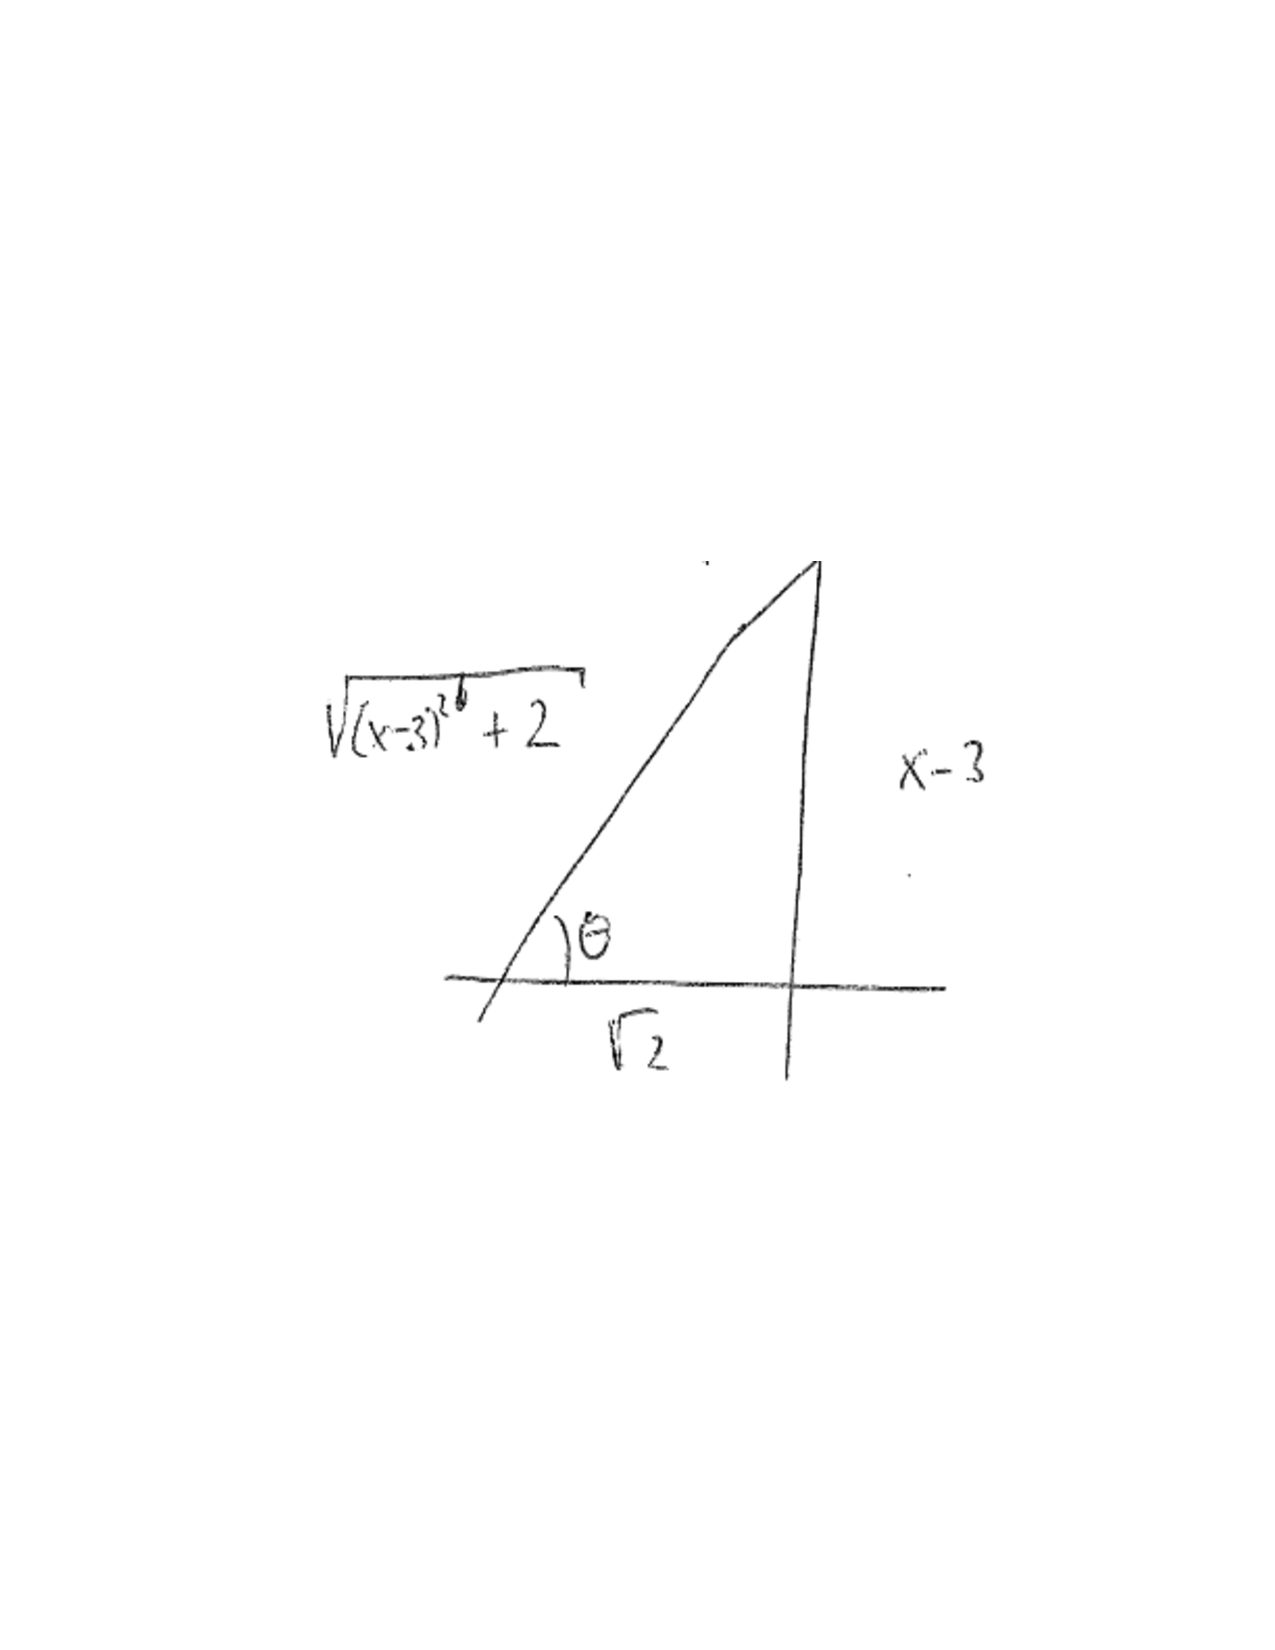
\includegraphics[trim= 230 270 250 280, scale=0.8]{Figure7-4-1.pdf}
		\end{image}
		
	Then we have that
		\[
		\sin(2\theta) = 2 \sin(\theta) \cos(\theta) = 2 \cdot \frac{x-3}{\sqrt{(x-3)^2+2}} \cdot \frac{\sqrt{2}}{\sqrt{(x-3)^2+2}}.
		\]
	Thus
		\[
		\int \frac{\d x}{\left( x^2 - 6x + 11 \right)^2} = \frac{\sqrt{2}}{8} \left( \arctan \left( \frac{x-3}{\sqrt{2}} \right) + \frac{\sqrt{2}(x-3)}{(x-3)^2+2} \right) + C .
		\]
	\end{freeResponse}
		
	\item 
	\[
	\int \frac{x^2}{\sqrt{4x-x^2}} \d x.
	\]
	\begin{freeResponse}
	Again, we begin by completing the square in the denominator, and then factoring
		\begin{align*}
		4x-x^2 &= -(x^2-4x)  \\
		&= -(x^2-4x+4) + 4  \\
		&= -(x-2)^2 + 4  \\
		&= 4 \left( - \frac{(x-2)^2}{4} + 1 \right)  \\
		&= 4 \left( 1 - \left( \frac{x-2}{2} \right)^2 \right).
		\end{align*}
	So
		\begin{align*}
		\int \frac{x^2}{\sqrt{4x-x^2}} \d x &= \int \frac{x^2}{\sqrt{4 \left( 1 - \left( \frac{x-2}{2} \right)^2 \right)}} \d x  \\
		&= \frac{1}{2} \int \frac{x^2}{\sqrt{1 - \left( \frac{x-2}{2} \right)^2}} \d x.
		\end{align*}
	We make the substitution
		\begin{equation}\label{substitution2}
		\frac{x-2}{2} = \sin \theta	\qquad	\Longrightarrow	\qquad	x = 2\sin \theta + 2
		\end{equation}
	which gives
		\[
		\d x = 2 \cos \theta \d \theta.
		\]
	Continuing with the integral, we have that
		\begin{align*}
		\frac{1}{2} \int \frac{x^2}{\sqrt{1 - \left( \frac{x-2}{2} \right)^2}} \d x
		&= \frac{1}{2} \int \frac{(2 \sin \theta + 2)^2}{\sqrt{1 - \sin^2 \theta}} \cdot 2 \cos \theta \d \theta  \\
		&= \int (2\sin \theta + 2)^2 \d \theta  \\
		&= \int ( 4 \sin^2 \theta + 8 \sin \theta + 4) \d \theta  \\
		&= \int (2(1-\cos(2\theta)) + 8\sin \theta + 4) \d \theta  \\
		&= \int (6 + 8\sin \theta - 2\cos(2\theta)) \d \theta  \\
		&= 6 \theta - 8 \cos \theta - \sin(2\theta) + C.
		\end{align*}
	Now all that is left to do is to reverse-substitute for $\theta$.  
	First, from equation \eqref{substitution2} we have that
		\[
		\theta = \arcsin \left( \frac{x-2}{2} \right).
		\]
	Now, we again use equation \eqref{substitution2} along with Pythagorean's Theorem to construct the following triangle.
	
		\begin{image}
		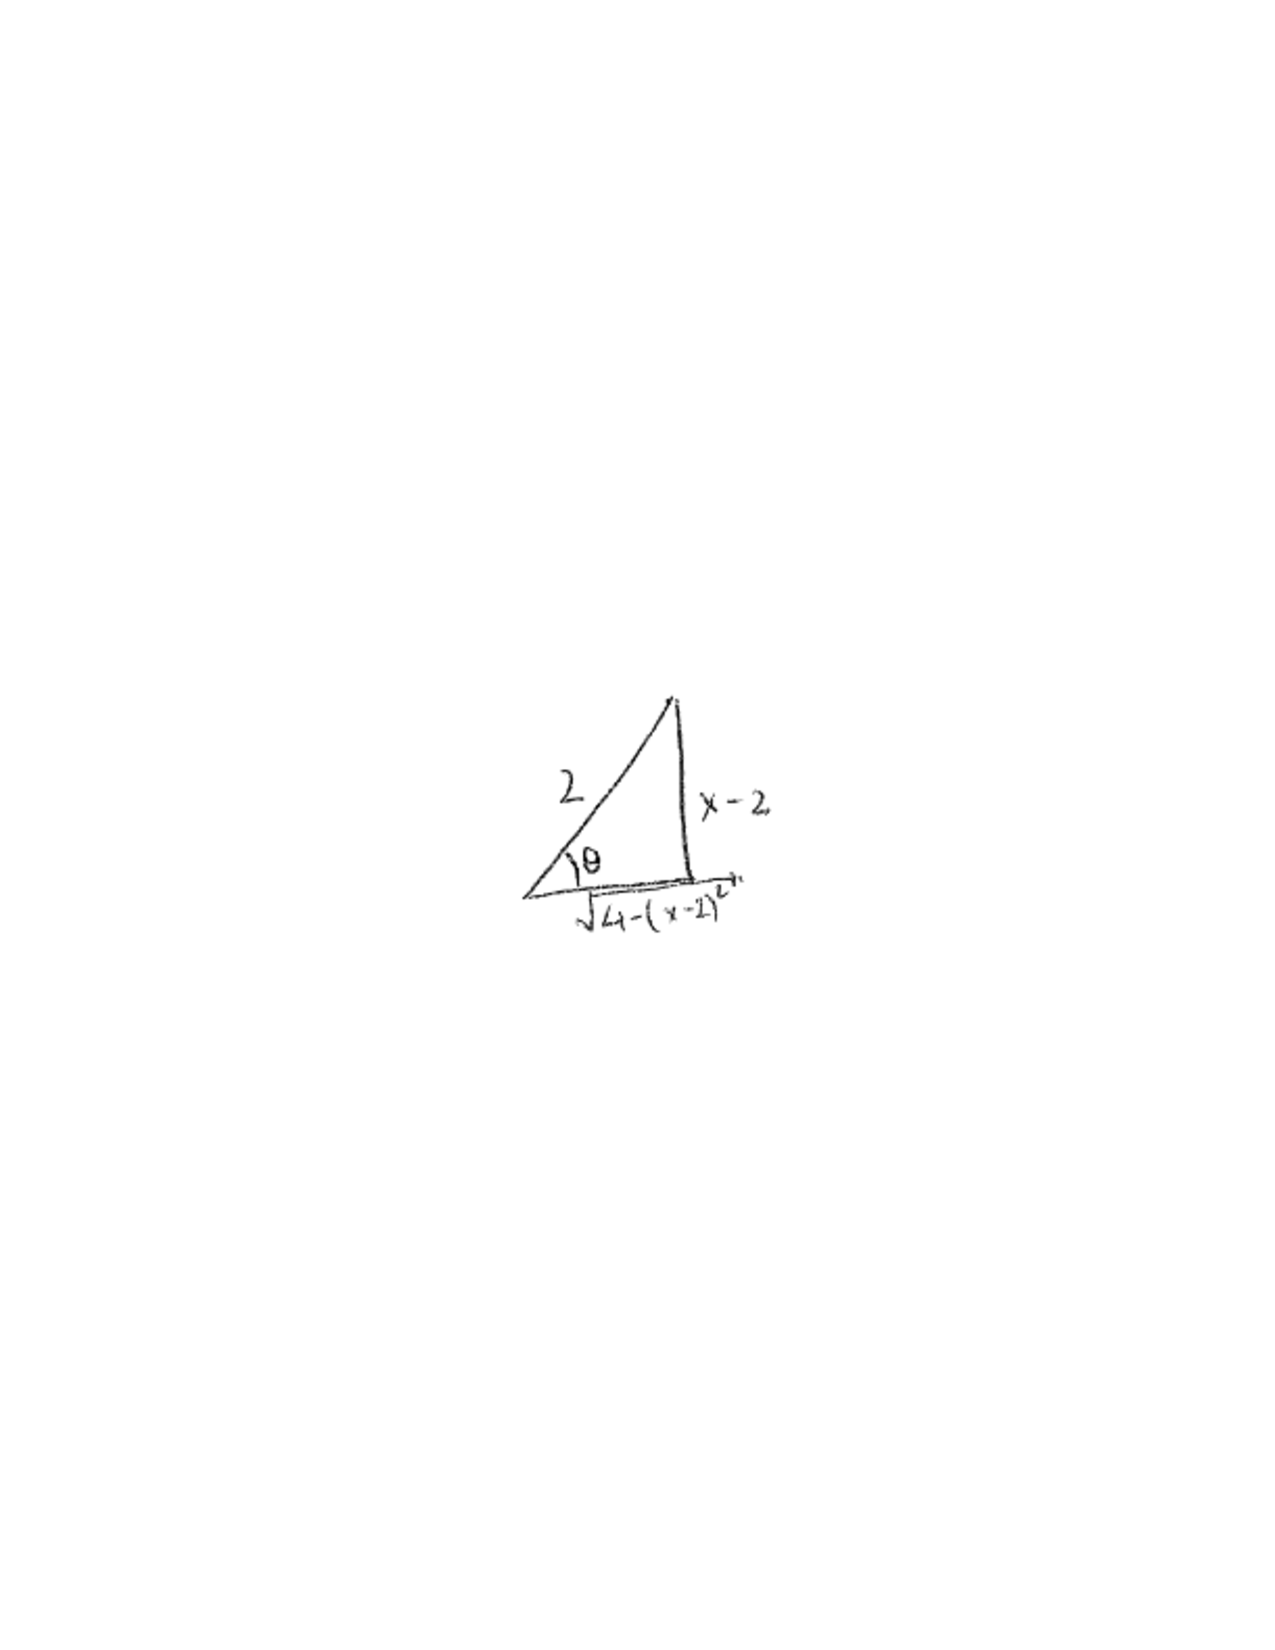
\includegraphics[trim= 270 350 250 330]{Figure7-4-2.pdf}
		\end{image}
		
	Then we have that
		\begin{align*}
		&\cos \theta = \frac{\sqrt{4-(x-2)^2}}{2}  \\
		&\sin(2\theta) = 2 \sin \theta \cos \theta = 2 \cdot \frac{x-2}{2} \cdot \frac{\sqrt{4-(x-2)^2}}{2}.
		\end{align*}
	Thus
		\[
		\int \frac{x^2}{\sqrt{4x-x^2}} \d x = 6\arcsin \left( \frac{x-2}{2} \right) - 4\sqrt{4-(x-2)^2} - \frac{(x-2)\sqrt{4-(x-2)^2}}{2}.
		\]
	\end{freeResponse}

	\item 
	\[
	\int \frac{e^x}{\sqrt{e^{2x}+9}} \d x.
	\]
	\begin{freeResponse}
	First, notice that
		\[
		\sqrt{e^{2x}+9} = \sqrt{9\left( \frac{e^{2x}}{9} + 1 \right)} = 3\sqrt{\left( \frac{e^x}{3} \right)^2 + 1}.
		\]
	So
		\[
		\int \frac{e^x}{\sqrt{e^{2x}+9}} \d x = \frac{1}{3} \int \frac{e^x}{\sqrt{\left( \frac{e^x}{3} \right)^2 + 1}} \d x.
		\]
	We make the substitution
		\begin{equation}\label{substitution3}
		\frac{e^x}{3} = \tan \theta 	\qquad	\Longrightarrow	\qquad	3\tan \theta = e^x
		\end{equation}
	which gives
		\[
		e^x \d x = 3 \sec^2 \theta \d \theta.
		\]
	Continuing with the integral, we have that
		\begin{align*}
		\frac{1}{3} \int \frac{e^x}{\sqrt{\left( \frac{e^x}{3} \right)^2 + 1}} \d x
		&= \frac{1}{3} \int \frac{1}{\sqrt{\tan^2 \theta + 1}} \cdot 3 \sec^2 \theta \d \theta  \\
		&= \int \sec \theta \d \theta  \\
		&= \ln | \sec \theta + \tan \theta | + C.
		\end{align*}
	Now all that is left to do is to reverse-substitute for $\theta$. 
	We use equation \eqref{substitution3} along with Pythagorean's Theorem to construct the following triangle.
	
		\begin{image}
		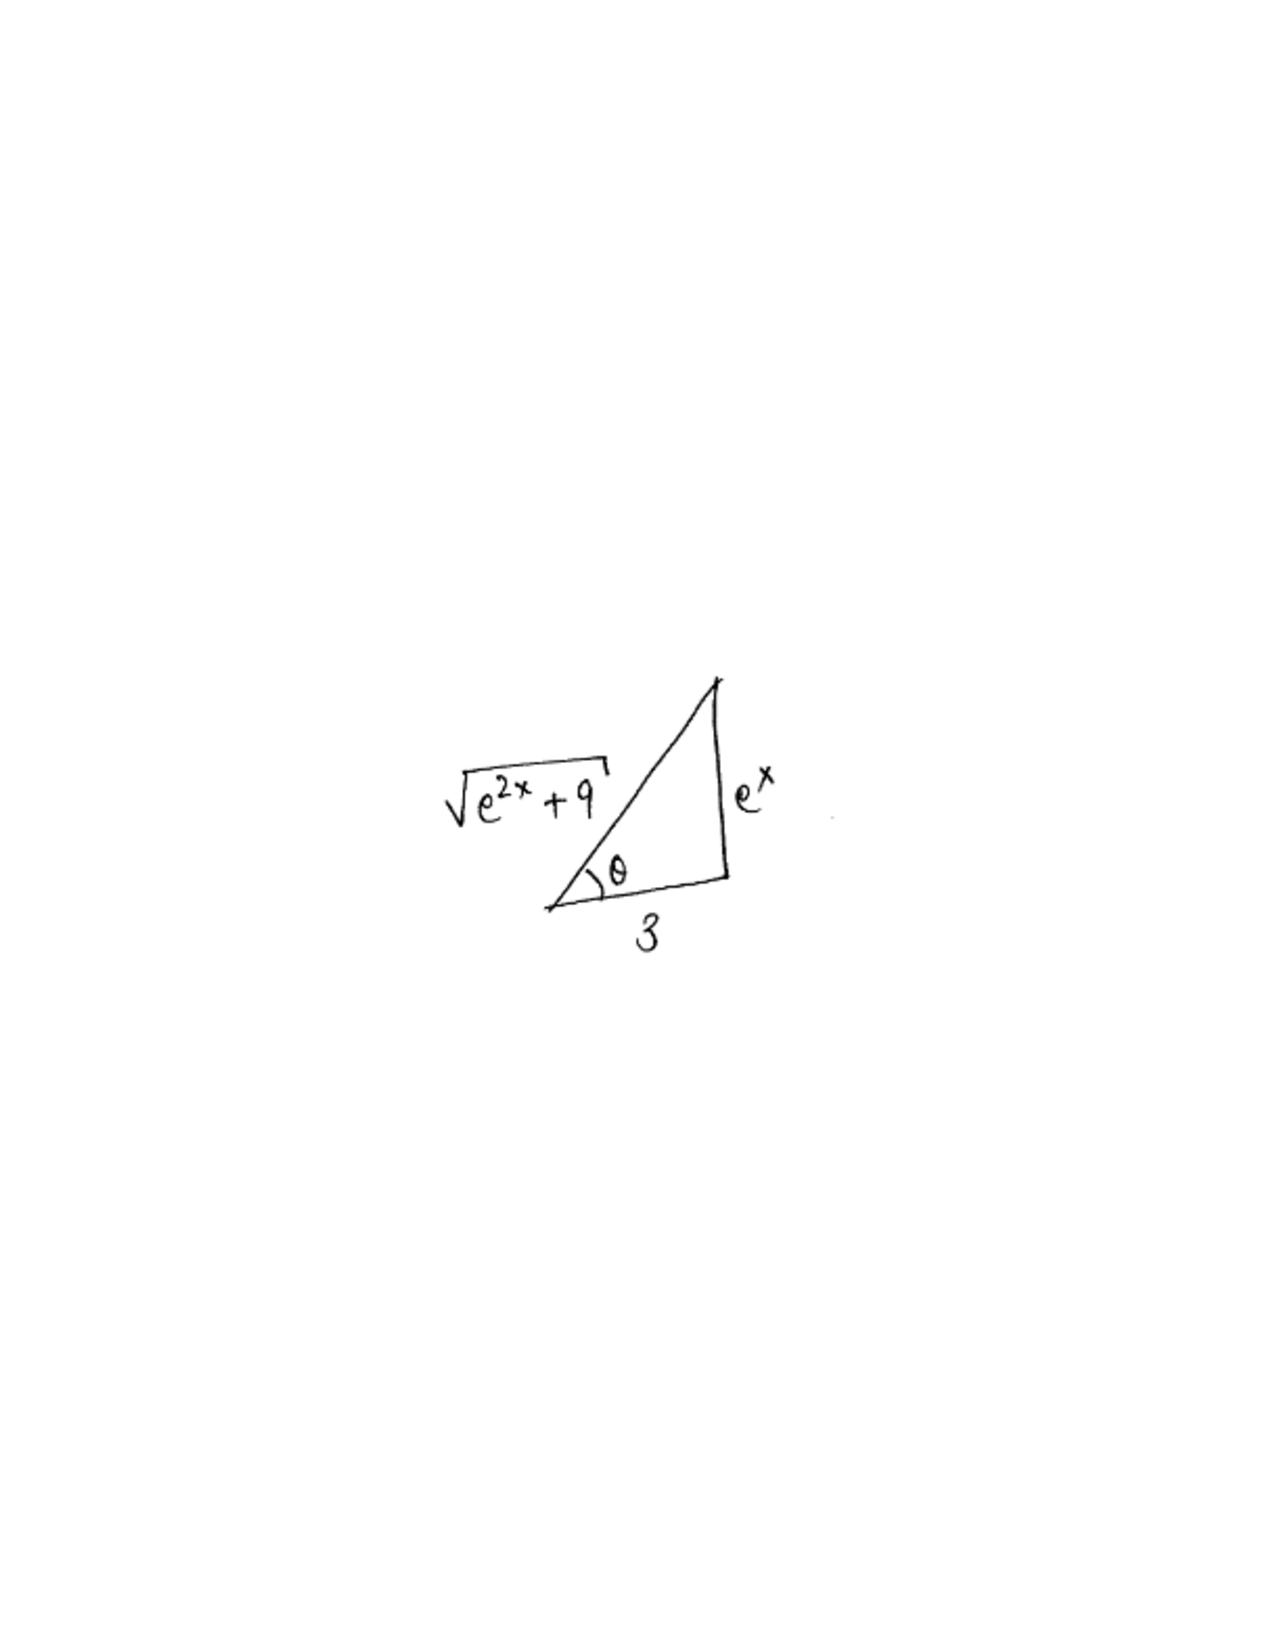
\includegraphics[trim= 270 350 250 330]{Figure7-4-3.pdf}
		\end{image}
		
	Then we have that
		\begin{align*}
		&\sec \theta = \frac{\sqrt{e^{2x}+9}}{3} \\
		&\tan \theta = \frac{e^x}{3}.
		\end{align*}
	Thus
		\[
		\int \frac{e^x}{\sqrt{e^{2x}+9}} \d x = \ln \left( \frac{\sqrt{e^{2x}+9} + e^x}{3} \right) + C.
		\]
	\end{freeResponse}



	\item 
	\[
	\int \frac{\d x}{x^{\frac{1}{2}} - 9x^{\frac{3}{2}}}.
	\]
	\begin{freeResponse}
		\begin{align*}
		\int \frac{\d x}{x^{\frac{1}{2}} - 9x^{\frac{3}{2}}}
		&= \int \frac{1}{x^{\frac{1}{2}} \left( 1 - 9x \right)} \d x  \\
		&= \int \frac{1}{x^{\frac{1}{2}} \left( 1 - \left( 3x^{\frac{1}{2}} \right)^2 \right)} \d x  \\
		&= \frac{2}{3} \int \frac{1}{1-u^2} \d x 	\qquad	{\color{red}\text{where }u=3x^{\frac{1}{2}}}  \\
		&= \frac{2}{3} \int \frac{1}{1-\sin^2 \theta} \cos \theta \d \theta	\qquad	{\color{red} \text{where } u=\sin \theta}  \\
		&= \frac{2}{3} \int \frac{\cos \theta}{\cos^2 \theta} \d \theta  \\
		&= \frac{2}{3} \int \sec \theta \d \theta  \\
		&= \frac{2}{3} \ln | \sec \theta + \tan \theta | + C  \\
		&= \frac{2}{3} \ln \left| \frac{1}{\sqrt{1-u^2}} + \frac{u}{\sqrt{1-u^2}} \right| + C  \\
		&= \frac{2}{3} \ln \left( \frac{1 + 3\sqrt{x}}{\sqrt{1-9x}} \right) + C
		\end{align*}
		
		\begin{image}
		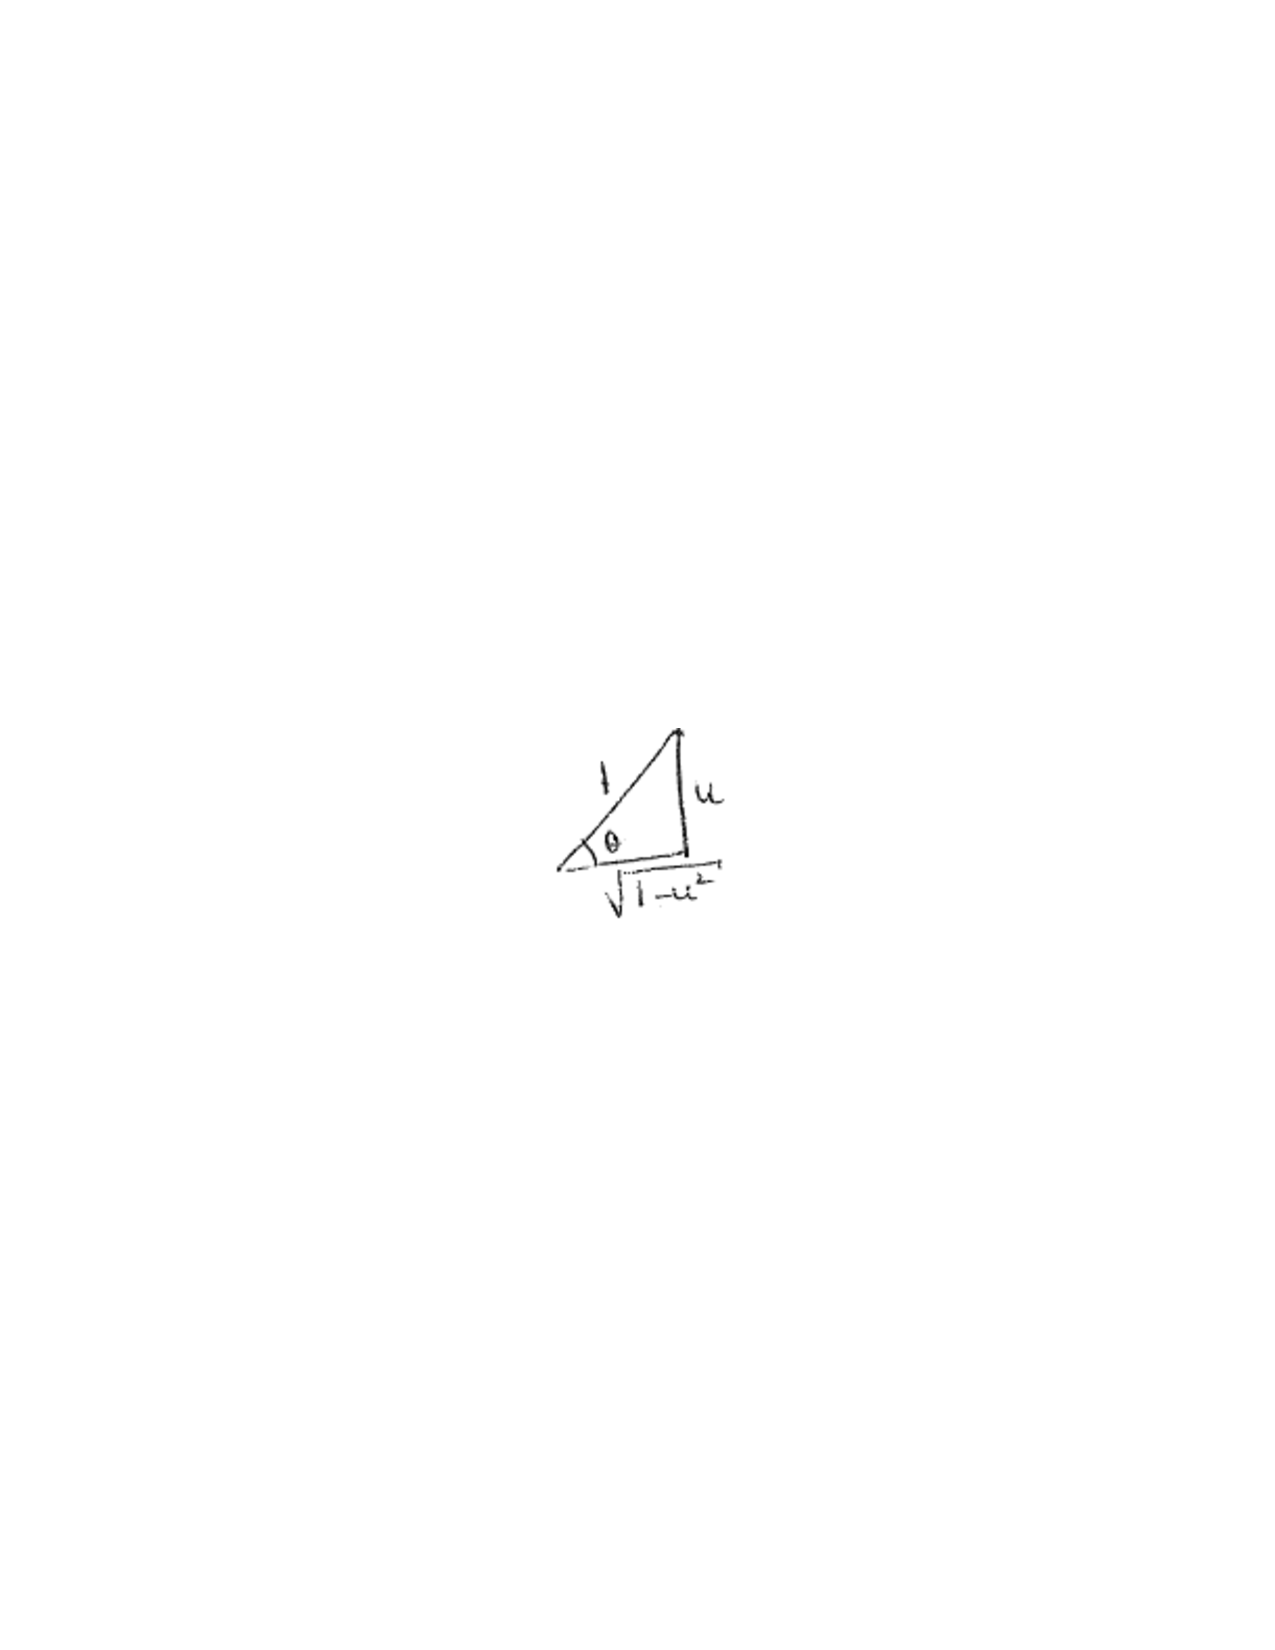
\includegraphics[trim= 270 350 250 360]{Figure7-4-4.pdf}
		\end{image}
		
	\end{freeResponse}

	\end{enumerate}

\end{problem}

\begin{instructorNotes}
Each of problems (a) through (c) involves one or more of the major points of trig substitution.  
Each of the three kinds of substitutions is represented, as well as working with absolute value issues in problem (a) (also could be brought up in problem (c)), completing the square, back substitution (c), and various trigonometric integrals.  
\dfn{Be adamant about substituting for $\d x$} as well as the rest of the integrand.  
In  (a), show the time-saving value of changing the limits in terms of $\theta$.  
\end{instructorNotes}
















	
	
	
	
	
	
	
	
	

	










								
				
				
	














\end{document} 


















